% Native editable composition from verified, unchanged IDE images.
\par
\begin{figure}[htbp]
\centering
\sbox0{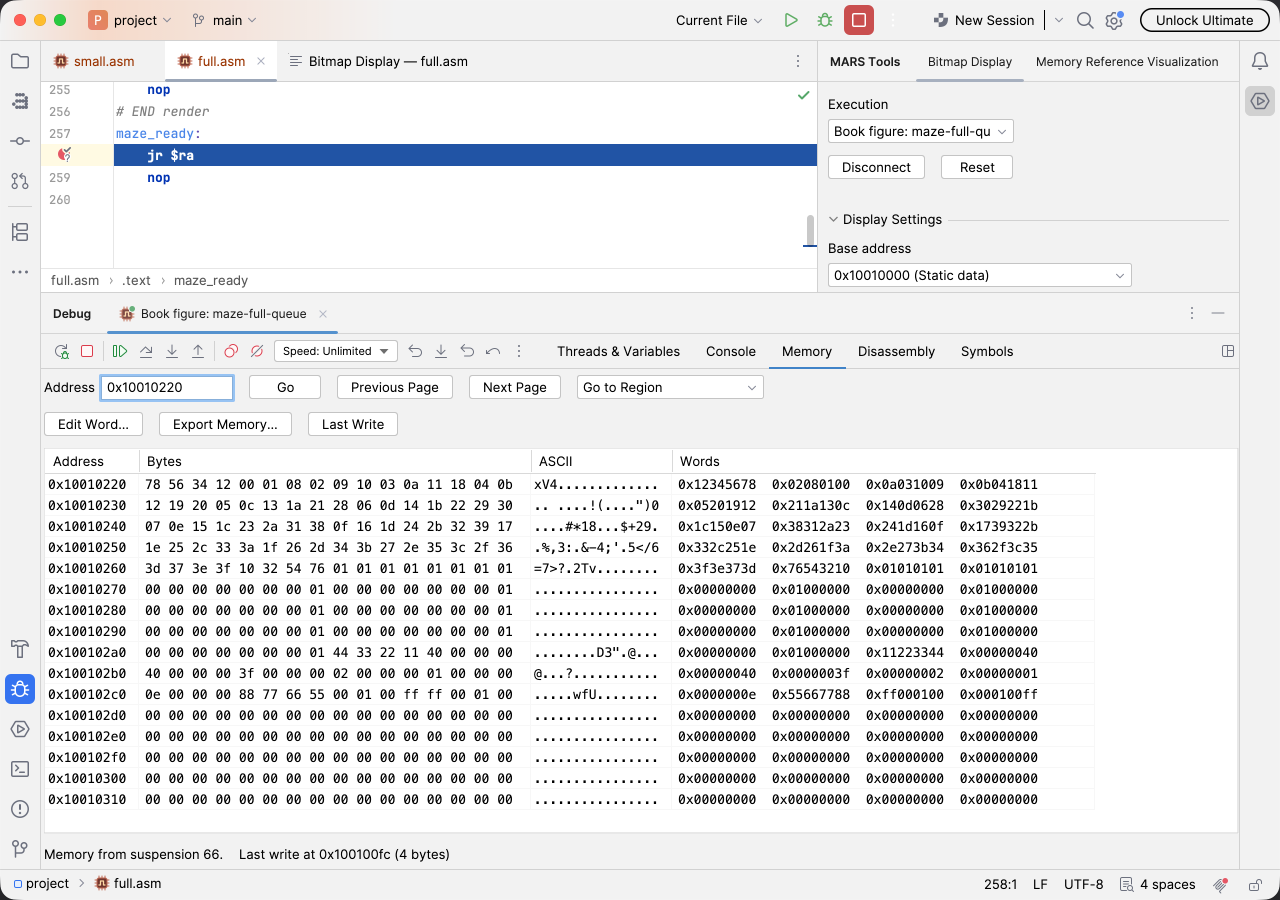
\includegraphics[artifact]{packages/010-maze-explorer/captures/f04-full/queue.png}}
\sbox2{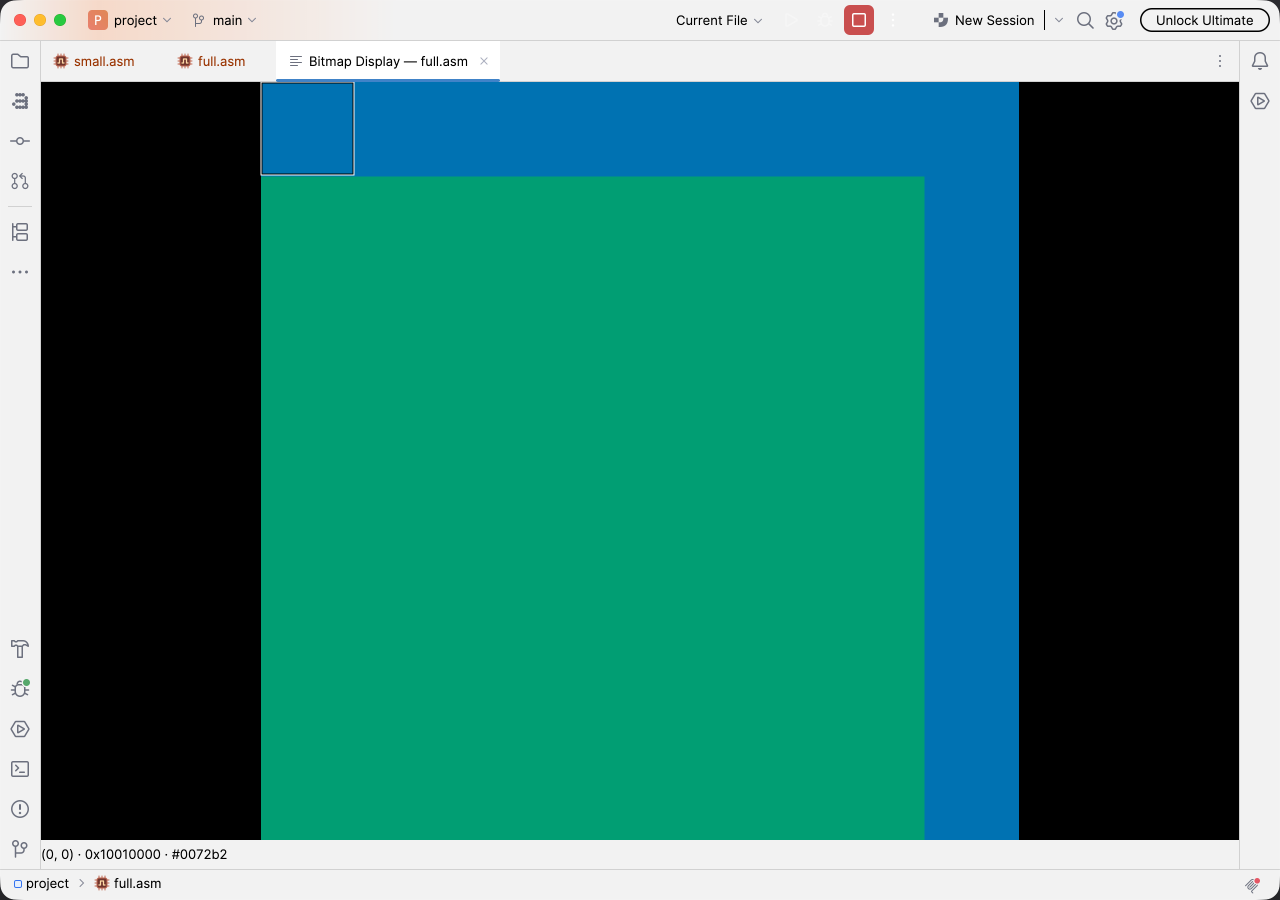
\includegraphics[artifact]{packages/010-maze-explorer/captures/f04-full/bitmap.png}}
\sbox4{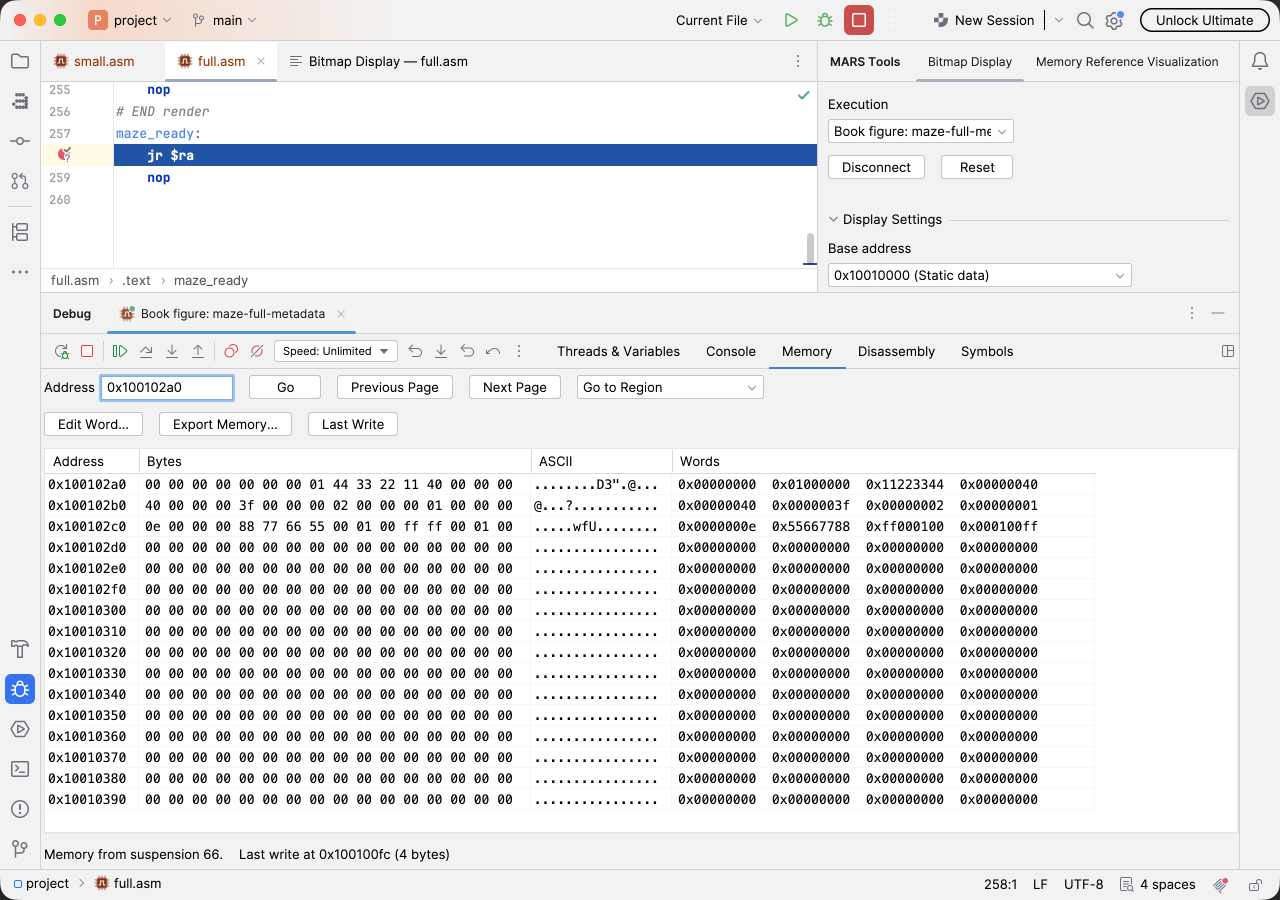
\includegraphics[artifact]{packages/010-maze-explorer/captures/f04-full/metadata.png}}
\edef\MARSfullsourceLeft{\the\dimexpr0.036718750\wd0\relax}
\edef\MARSfullsourceBottom{\the\dimexpr0.811111111\ht0\relax}
\edef\MARSfullsourceRight{\the\dimexpr0.611718750\wd0\relax}
\edef\MARSfullsourceTop{\the\dimexpr0.111111111\ht0\relax}
\edef\MARSfullstateLeft{\the\dimexpr0.034375000\wd0\relax}
\edef\MARSfullstateBottom{\the\dimexpr0.352222222\ht0\relax}
\edef\MARSfullstateRight{\the\dimexpr0.584375000\wd0\relax}
\edef\MARSfullstateTop{\the\dimexpr0.497777778\ht0\relax}
\edef\MARSfullplotLeft{\the\dimexpr0.203906250\wd2\relax}
\edef\MARSfullplotBottom{\the\dimexpr0.066666667\ht2\relax}
\edef\MARSfullplotRight{\the\dimexpr0.203906250\wd2\relax}
\edef\MARSfullplotTop{\the\dimexpr0.091111111\ht2\relax}
\edef\MARSfullmemoryLeft{\the\dimexpr0.034375000\wd4\relax}
\edef\MARSfullmemoryBottom{\the\dimexpr0.398888889\ht4\relax}
\edef\MARSfullmemoryRight{\the\dimexpr0.584375000\wd4\relax}
\edef\MARSfullmemoryTop{\the\dimexpr0.497777778\ht4\relax}
\begin{tikzpicture}[alt={Four annotated details for an open eight by eight room with goal sixty-three. Queue storage contains sixty-four distinct cell IDs, including goal sixty-three in the last slot. The route follows all eight top-row cells and then the seven remaining right-column cells, giving fifteen cells and fourteen edges. Head and tail are sixty-four, phase two, result one and length fourteen.}]
\node[anchor=north west,inner sep=0,font=\small\bfseries] (source-title) at (6mm,0) {Next instruction: return from the renderer};
\node[anchor=north west,inner sep=0] (source) at ([yshift=-1mm]source-title.south west) {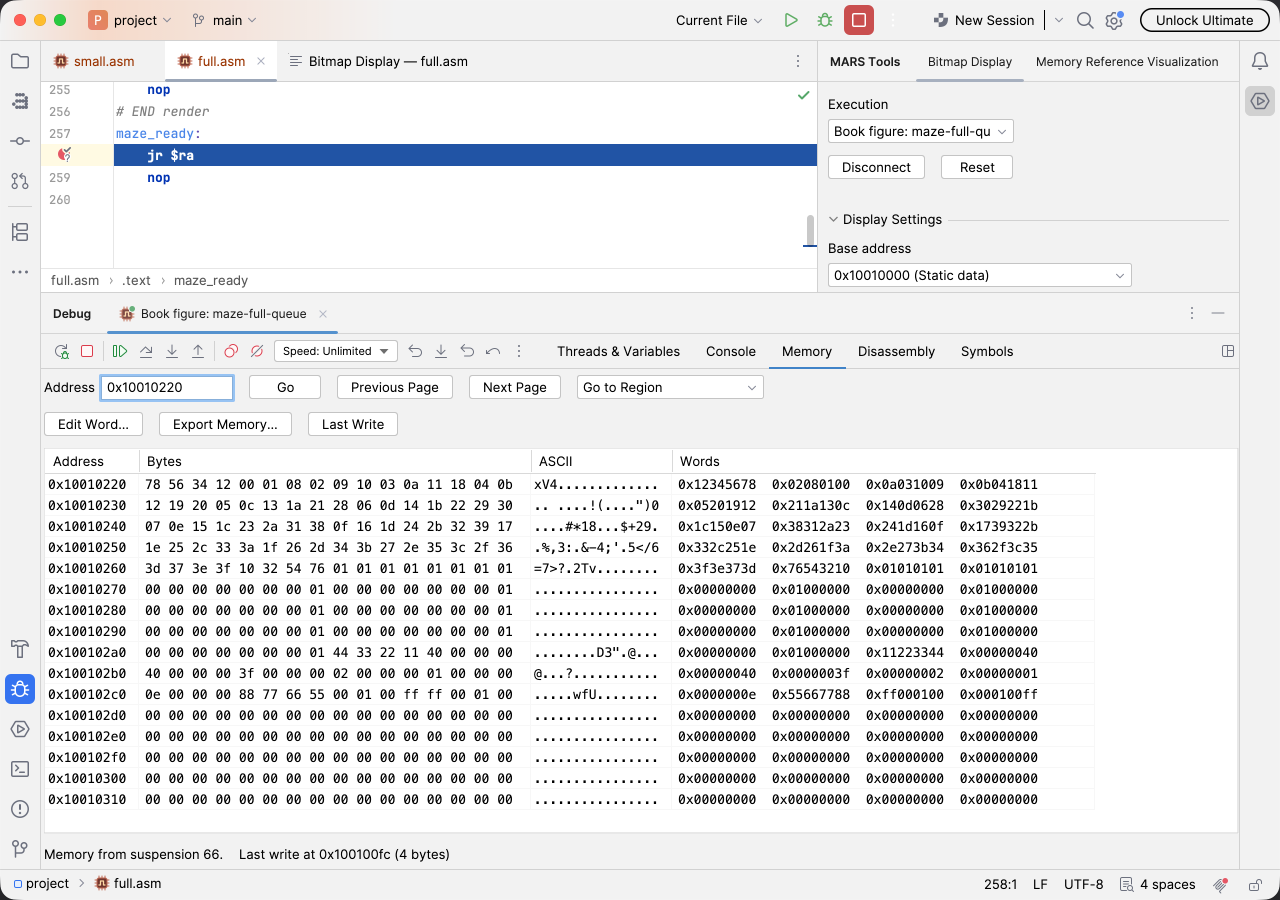
\includegraphics[width=0.7\linewidth,artifact,trim={\MARSfullsourceLeft{} \MARSfullsourceBottom{} \MARSfullsourceRight{} \MARSfullsourceTop{}},clip]{packages/010-maze-explorer/captures/f04-full/queue.png}};
\begin{scope}[shift={(source.south west)},x={($(source.south east)-(source.south west)$)},y={($(source.north west)-(source.south west)$)}]
\draw[black,line width=0.7pt] (0.153333333,0.057142857) rectangle (0.326666667,0.371428571);
\node[draw=black,fill=white,circle,inner sep=1.5pt,font=\footnotesize] at ($(0.153333333,0.371428571)+(-3mm,0)$) {1};
\end{scope}
\node[anchor=north west,inner sep=0,font=\small\bfseries] (state-title) at ([yshift=-1mm]source.south west) {All 64 queue-history bytes};
\node[anchor=north west,inner sep=0] (state) at ([yshift=-1mm]state-title.south west) {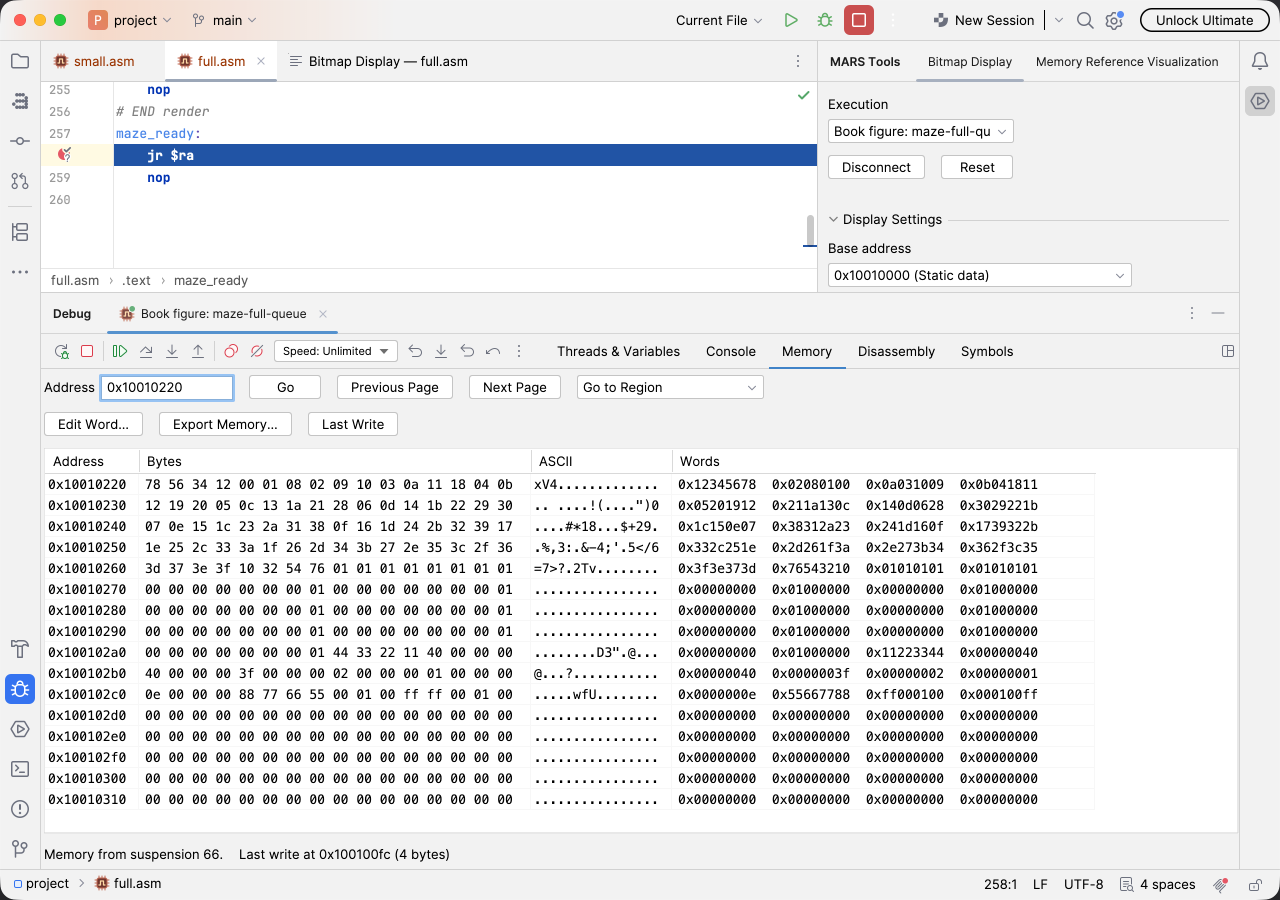
\includegraphics[width=0.65\linewidth,artifact,trim={\MARSfullstateLeft{} \MARSfullstateBottom{} \MARSfullstateRight{} \MARSfullstateTop{}},clip]{packages/010-maze-explorer/captures/f04-full/queue.png}};
\begin{scope}[shift={(state.south west)},x={($(state.south east)-(state.south west)$)},y={($(state.north west)-(state.south west)$)}]
\draw[black,line width=0.7pt] (0.194672131,0.029629630) rectangle (0.997950820,0.807407407);
\node[draw=black,fill=white,circle,inner sep=1.5pt,font=\footnotesize] at ($(0.000000000,0.807407407)+(-3mm,0)$) {2};
\end{scope}
\node[anchor=north west,inner sep=0,font=\small\bfseries] (plot-title) at ([xshift=0.69\linewidth]state-title.north west) {Complete published maze};
\node[anchor=north west,inner sep=0] (plot) at ([yshift=-1mm]plot-title.south west) {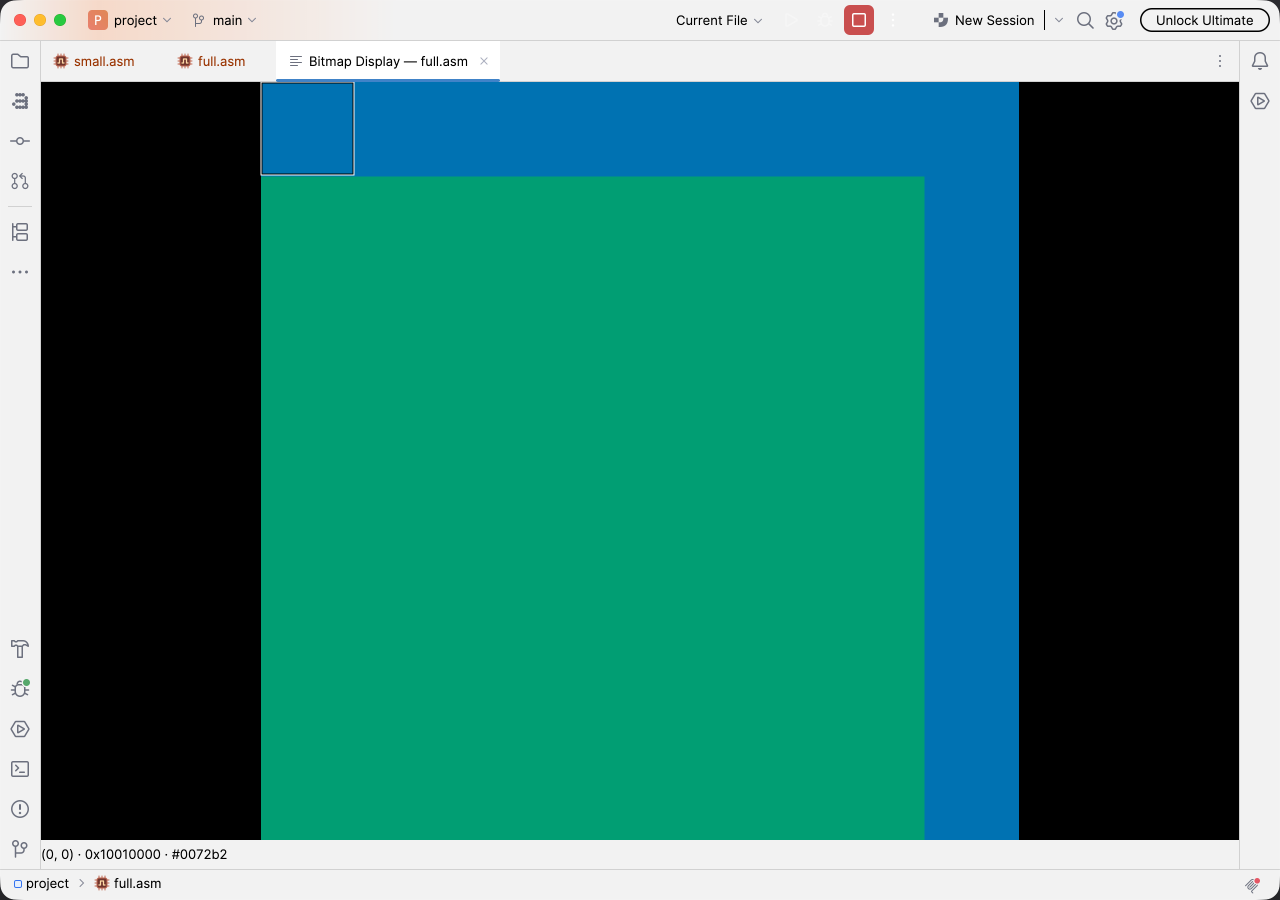
\includegraphics[width=0.27\linewidth,artifact,trim={\MARSfullplotLeft{} \MARSfullplotBottom{} \MARSfullplotRight{} \MARSfullplotTop{}},clip]{packages/010-maze-explorer/captures/f04-full/bitmap.png}};
\begin{scope}[shift={(plot.south west)},x={($(plot.south east)-(plot.south west)$)},y={($(plot.north west)-(plot.south west)$)}]
\draw[black,line width=0.7pt] (0.000000000,0.000000000) rectangle (1.000000000,1.000000000);
\node[draw=black,fill=white,circle,inner sep=1.5pt,font=\footnotesize] at ($(0.000000000,1.000000000)+(-3mm,0)$) {3};
\foreach \c in {0,...,7} {\node[anchor=north,font=\scriptsize,inner sep=0] at ({(\c+0.5)/8},-0.035) {\c}; \node[anchor=east,font=\scriptsize,inner sep=0] at (-0.025,{1-(\c+0.5)/8}) {\c};}
\node[anchor=north,font=\scriptsize,inner sep=0] at (0.5,-0.11) {$x$}; \node[anchor=east,font=\scriptsize,inner sep=0] at (-0.10,0.5) {$y$};
\end{scope}
\node[anchor=north west,inner sep=0,font=\small\bfseries] (memory-title) at ([yshift=-9mm]state-title.north west |- plot.south west) {Queue counters and final result};
\node[anchor=north west,inner sep=0] (memory) at ([yshift=-1mm]memory-title.south west) {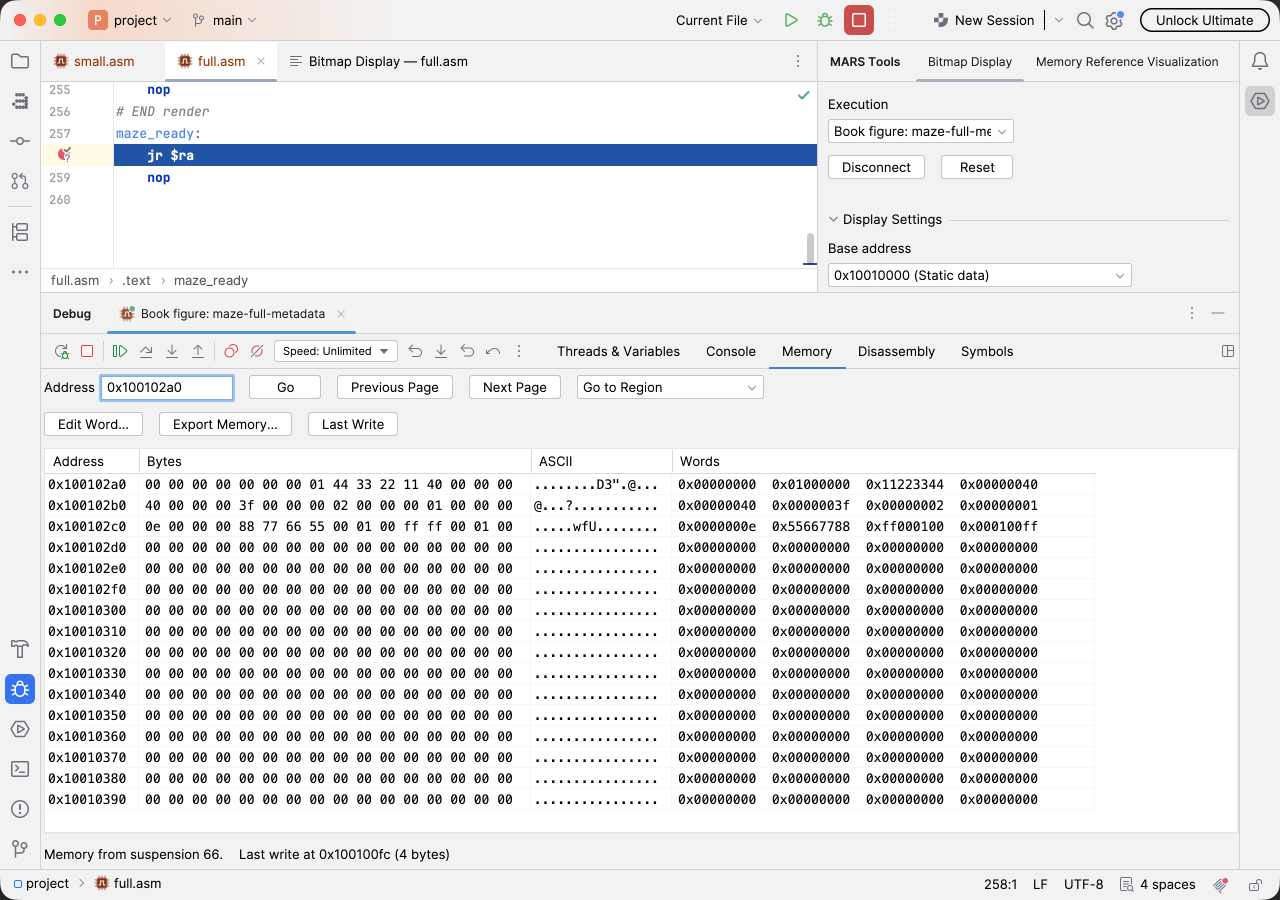
\includegraphics[width=0.78\linewidth,artifact,trim={\MARSfullmemoryLeft{} \MARSfullmemoryBottom{} \MARSfullmemoryRight{} \MARSfullmemoryTop{}},clip]{packages/010-maze-explorer/captures/f04-full/metadata.png}};
\begin{scope}[shift={(memory.south west)},x={($(memory.south east)-(memory.south west)$)},y={($(memory.north west)-(memory.south west)$)}]
\draw[black,line width=0.7pt] (0.194672131,0.043010753) rectangle (0.997950820,0.720430108);
\node[draw=black,fill=white,circle,inner sep=1.5pt,font=\footnotesize] at ($(0.000000000,0.720430108)+(-3mm,0)$) {4};
\end{scope}
\end{tikzpicture}
\par\smallskip
\begin{minipage}{\linewidth}
\small
\begin{enumerate}
\item This fixture changes only the walls data and goal word; the instructions are unchanged. \texttt{word(phase) == 2} selects its final publication at the same renderer-return boundary.
\item Queue bytes occupy \texttt{0x10010224} through \texttt{0x10010263}. All 64 slots retain distinct discovered cell IDs. The final byte is \texttt{3f} (cell 63); the following guard begins at \texttt{0x10010264}. Zero in the first slot is a valid cell ID.
\item The selected route follows row 0 from columns 0 through 7, then column 7 through rows 1 through 7. Its fifteen blue cells use fourteen edges. The other 49 cells are processed green cells; none are walls or pending frontier cells.
\item The bytes \texttt{40 00 00 00} encode decimal 64 for both head and tail. The active interval is empty, although the storage history fills the allocation. Current is 63, phase 2, result 1, and length \texttt{0e} is decimal 14. No store targets queue slot 64.
\end{enumerate}
\end{minipage}
\caption{All queue slots retain discovery history while the final active frontier is empty.}
\label{capture:010-maze-explorer-f04-full}
\label{maze-f04-full}
\end{figure}
\par
